\subsection{Uvod v LaTeX}

\subsubsection{Kaj je LaTeX?}\label{latexUvod_kajJeLaTeX}

LaTeX je program za oblikovanje besedil.
LaTeX je nadgradnja programa TeX, ki je razvil Donald E. Knuth. leta 1997.
Prvo verzijo LaTeX-a je napisal Leslie Lamport (1980). LaTeX je paket dodatnih ukazov za TeX, ki avtorjem omogočajo oblikovanje in izpisovanje dokumentov v najvišji kvaliteti s pomočjo že pripravljenih profesionalnih vzorcev.

Trenutna standardna verzija je LaTeX2e (1994), zanj pa je odgovoren Frank Mittelbach. LaTeX se izgovori `láteh', po angleško pa običajno rečemo `lejteh'.

Ko želi \textit{avtor} kaj objaviti, pošlje svoj rokopis založniku.
Tam \textit{knjiži opremljevalec} določi obliko dokumenta (širino stolpcev, obliko črk, velikost presledkov pred in po naslovih ... ).
Opremljevalec svoja navodila skupaj z rokopisom preda \textit{črkostavcu}, ki na podlagi teh podatkov stavi knjigo.
V LaTeX-u prevzame vlogi knjižnega oblikovalca in črkostavca, da se avtor osredotoči na vsebino Figure~\ref{kaj-je-latex}.

\begin{figure}[!htbp]
\centering
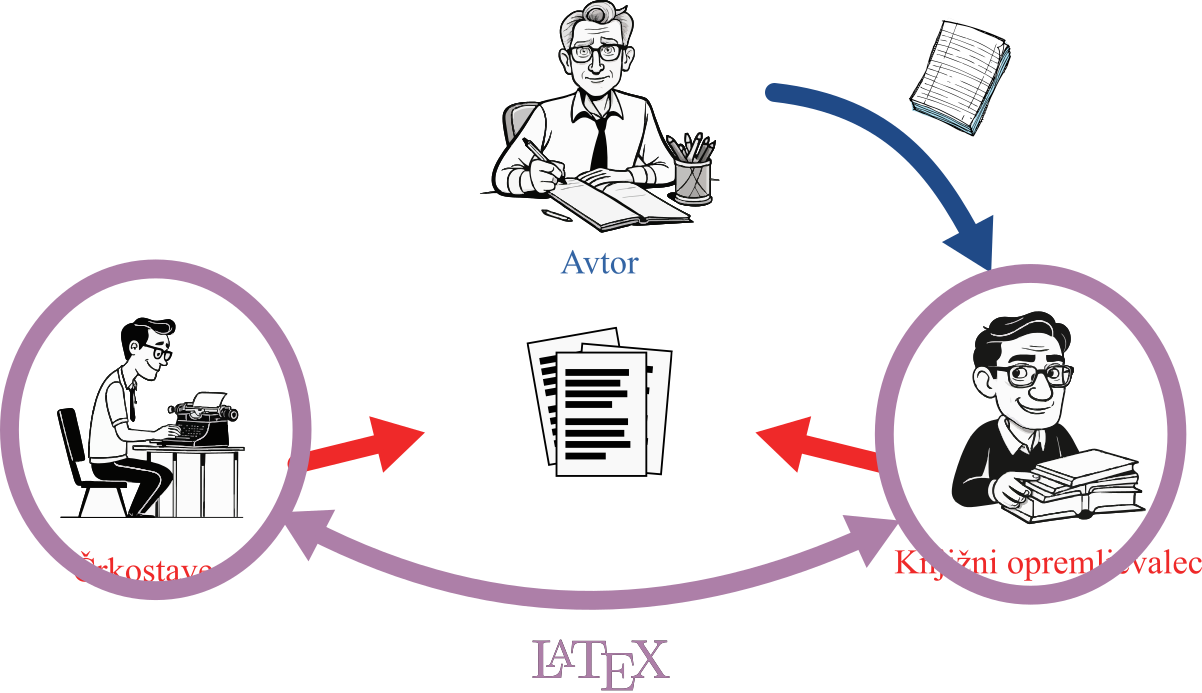
\includegraphics[width=0.8\linewidth]{files/01_osnovne-6aebd97826dc992bdf7f8e18b95c6a57.png}
\caption[]{Kaj je LaTeX?}
\label{kaj-je-latex}
\end{figure}

\begin{framed}
\textbf{Pomebno: Filozofija LaTeXa}\\
Oblikovanje dokumentov z LaTeXom sledi naslednjemu načelu:

\begin{quote}
mi (avtorji) se ukvarjamo z \textbf{vsebino} dokumenta, LaTeX pa poskrbi za \textbf{oblikovanje}.
\end{quote}

Ali, enakovredno,

\begin{quote}
ne skrbimo za \textbf{oblikovanje}, zato se lahko osredotočimo na \textbf{vsebino}.
\end{quote}
\end{framed}

\subsubsection{Kaj zmore LaTeX?}\label{latexUvod_KajZmoreLaTeX}

LaTeX zmore skoraj vse, kar zmorejo drugi urejevalniki besedil.
Vendar pa je LaTeX posebej primeren za pisanje znanstvenih in tehničnih besedil, ki vsebujejo veliko matematičnih formul in simbolov.
LaTeX omogoča tudi enostavno ustvarjanje tabel, grafov in drugih elementov, ki so pogosto potrebni v tehničnih besedilih.
Poleg tega LaTeX omogoča enostavno ustvarjanje kazal, bibliografij in drugih elementov, ki so pomembni za znanstvena besedila.

Čeprav je LaTeX optimiziran za izdelavo znanstvenih in tehničnih besedil, ni omejen samo na to. Danes uporabljam LaTeX za pisanje vseh dokumentov, ki naj izgledajo profesionalno ali lepo.
To sega od osebnih in poslovnih pisem do pesmarice za igranje kitare.

Vprašal sem moje sodelavce, kaj delajo z LaTeXom.
Tukaj je nekaj zanimivih odgovorov:

\begin{itemize}
\item Knjnige, članke, in zapiski predavanj;
\item Predstavitve, s pomočjo Beamer-ja \href{/latexbeamer}{Beamer: Prestavitve v LaTeXu};
\item Profesionalna dokumentacija (npr CV, projekte vloge);
\item Pogodbe za stanovanje;
\item Pisma;
\item Pravila za družabne igre
\item Note (za glasbo)
\item Facebook, SMS, Instagram (da, res je!).
\item \textbf{Zaključna dela (diplome, magistrska, doktorat)}
\end{itemize}

Če vas zanima, si lahko tukaj ogledate \href{https://anteromontonio.github.io/assets/pdf/2019\_Mon\_phDThesis.pdf}{mojo doktorsko disertacijo}, ki je bila napisana izključno z uporabo programa LaTeX.

\subsubsection{LaTeX ni Word}\label{latexUvod_latexNiWord}

MS Word, Google Docs, LibreOffice, so WYSIWYG (kar vidiš, to tudi dobiš).
V teh programih avtor obliko dokumenta določi interaktivno med samim vnosom besedila v računalnik. Med celotnim procesom na zaslonu vidi, kakšna bo končna oblika, ko bo dokument natisnjen.

Pri LaTeXu ni možno videti končne oblike med samim tipkanjem besedila.
Lahko pa vidimo končno obliko na zaslonu, potem ko datoteko prevedemo z LaTeXom.
Tako lahko popravke naredimo še preden dokument izpišemo s tiskalnikom.
V urejevalnikih WYSIWYG strukturo in obliko urejate hkrati z pisanjem besedila.
Zlasti pri dolgih projektih se je zelo lahko izgubiti.
LaTeX sili avtorja, da določi logično strukturo besedila, LaTeX pa potem izbere najprimernejšo obliko.

\paragraph{Zakaj LaTeX?}\label{latexUvod_zakaj}

Predstavljajmo si, da pišete roman v svojem najljubšem urejevalniku WYSIWYG.
V tej knjigi se odvijata dve vzporedni zgodbi v
različnih dimenzijah.
Da bi bralcu sporočili, katera od dimenzij je trenutno opisana, ste se odločili, da boste za obe uporabili različne barve.
Vaša knjiga bi tako lahko izgledala takole:

„Ne, ne moreš me zapustiti!`` je zaklical  Peredur Lancelotu.\newline
„Moram,`` je odgovoril. „Usoda me kliče. Toda ponovno se bova srečala. Obljubim.``

Shao je občutila nepojasnjeno žalost, kot da bi pravkar izgubila nekaj ali nekoga, ki ji je bil pomemben.\newline
„Si v redu?`` je vprašala Ashby, medtem ko je jedla svojo kašo.\newline
„Ne izgledaš dobro.``\newline
„V redu sem, samo utrujena.``

Ko ste končali prvi osnutek (ki obsega 300 strani), ste se odločili, da ga pošljete po e-pošti prijatelju, da vam bo povedal svoje mnenje.
Vendar se je izkazalo, da lahko tiskalnik vašega prijatelja tiska samo črno-belo, zato ne more natisniti datoteke, ki ste mu jo poslali.

Enostavna rešitev! Vse zeleno besedilo spremenite v kursivno pisavo, ostalo pa pustite v pisavi upright front.
Po ročni spremembi vsakega odstavka prvih 120 strani knjige ste se spomnili, da v nekaterih primerih za poudarjanje uporabljate kursivno pisavo:
[Ali boš \textit{to} jedla?]\{.latex-line .text-green\}
Sedaj boste morali preveriti vsak odstavek za kurzivo in ga spremeniti v drug slog, preden spremenite vse zeleno besedilo v kurzivo.

\textbf{Vidite neskončni problem?}.

LaTeX rešuje ta problem tako, da avtorju omogoča, da se osredotoči na vsebino in logično strukturo besedila, medtem ko LaTeX poskrbi za oblikovanje.

\subsubsection{Kako deluje LaTeX?}\label{latexUvod_kakoDeluje}

Klasična razlaga delovanja LaTeX-a je naslednja:

\begin{enumerate}
\item Avtor napiše besedilo in ukaze LaTeX v datoteko \texttt{.tex} (npr. \texttt{ime\_datoteke.tex}).
\item Datoteka \texttt{.tex} prevedemo z LaTeX-om, ki ustvari datoteko \texttt{.dvi} (npr. \texttt{ime\_datoteke.dvi}).
\item Datoteke \texttt{.dvi} niso standardne, zato je treba datoteka \texttt{.dvi} pogosto spremeniti v datoteko \texttt{.pdf}; na koncu dobimo datoteko \texttt{ime\_datoteke.pdf}, ki jo lahko natisnemo ali delimo z drugimi.
\end{enumerate}

V sodobnem času pogosto gremo iz \texttt{ime\_datoteke.tex} datoteke neposredno v \texttt{ime\_datoteke.pdf}\} npr. z pomočijo programa \texttt{pdflatex}.

\begin{figure}[!htbp]
\centering
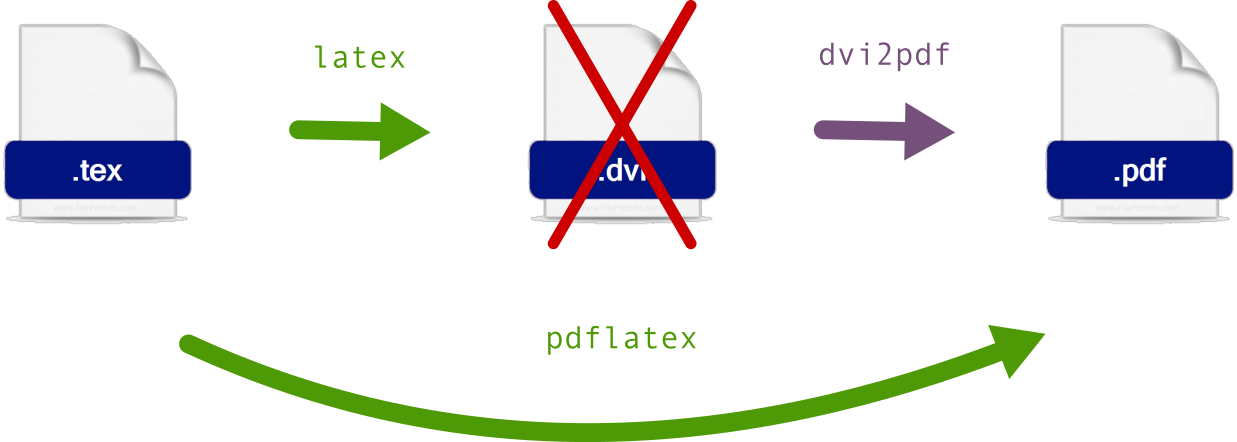
\includegraphics[width=0.8\linewidth]{files/01_datoteke-7b4841f3665416115ad84e4cf891a1cb.png}
\caption[]{Kajo deluje LaTeX?}
\label{kako-deluje-latex}
\end{figure}

\subsubsection{Kako začeti z LaTeXom?}\label{latexUvod_kakoZaceti}

Lahko namestite na svoj računalnik.
Če vas to želite, poglejte \href{/a-namescanjelatexa}{Nameščanje LaTeXa na svoj računalnik}.

Uporabili bomo drugačen pristop in delali z LaTeXom na spletu.
To bomo storili prek Overleaf, ki je platforma za delo z LaTeX projekti na spletu.
Najprej morate ustvariti račun.

%  ## Prva datoteka v LaTeXu

\subsubsection{Ukazi in okolja}

Kot smo že~omenili, se moramo pri delu z LaTeXom osredotočiti na vsebino, oblikovanje pa prepustiti LaTeXu.
Ker pa je LaTeX ``samo'' računalniški program, potrebuje
več vodenja.
Avtor mora navesti dodatne informacije, ki opisujejo logično strukturo njegovega dela.
Te informacije se navedejo prek \textit{ukazov} in \textit{okolij}, ki se vpišejo okoli besedila.

Ukazi v LaTeXu imajo splošno obliko:

\begin{verbatim}
\imeUkaza[neobvezni argument]{argument}
\end{verbatim}

in se običajno uporablja za dajanje LaTeXu določenih navodil.

\begin{itemize}
\item Ukaz \textit{vedno} se začne z znakom \texttt{{\textbackslash}}.
\item Argumentov je lahko več, npr. \texttt{\{prvi\}\{drugi\}...\{zadnji\}} ali  nobenega (npr. ukaz \texttt{{\textbackslash}tiny}, vendar je to redko).
\item Lahko je več neobveznih argumentov: \texttt{[prvi, drugi, ..., zadnji]}  ali noben (in potem ne napišemo ničesar). Pazite razliko z \texttt{obveznimi argumenti}.
\end{itemize}

Okolje je posebna vrsta ukaza z naslednjo strukturo:

\begin{verbatim}
\begin{okolje}
  Vsebina okolja: ukazi in besedilo
\end{okolje}
\end{verbatim}

Okolja običajno nadzorujejo, kako se bo del besedila/kode obnašal, ko bo natisnjen v dokument.

Zaenkrat vam ni treba skrbeti, kako delujejo ukazi in okolja.
To bomo spoznavali sproti.
V poglavju \href{/latexosnovnaokolja}{Osnovna okolja}  bomo podrobneje pogledali nekatera najpomembnejša okolja.

\subsubsection{Preambula in telo datoteke}\label{latexUvod_preambulaTelo}

Vsaka datoteka LaTeX ima naslednjo obliko:

\begin{verbatim}
%Preambula
\documentclass{...}
\usepackage{...}
%... 
% Telo
\begin{document}
  Vsebina dokumenta.
\end{document}
\end{verbatim}

Najpomembnejše okolje v lateksu je okolje \texttt{document}.
To okolje se lahko uporabi največ enkrat na dokument in v tem okolju pa napišemo dejansko vsebino našega dokumenta.
Vse, kar je znotraj tega okolja, se imenuje \textit{telo} dokumenta.

Če je najpomembnejše okolje \texttt{document}, mora biti najpomembnejši ukaz \texttt{{\textbackslash}documentclass}.
Vse, kar je med ukazom \texttt{{\textbackslash}documentclass} in začetkom okolja \texttt{document}, se imenuje \textit{preambula} dokumenta.
Tukaj nadzorujemo splošno delovanje LaTeXa.

\begin{framed}
\textbf{Opozirilo!}\\
Preambula običajno vsebuje samo ukaze (v nasprotju z običajnim besedilom) in obstajajo ukazi, ki se lahko uporabljajo samo v preambuli.
Pogosta napaka v LaTeXu je, da se del kode napiše na napačno mesto.
\end{framed}

Ukaz \texttt{{\textbackslash}documentclass} določa vrsto dokumenta, ki ga želimo ustvariti.
Uporabljamo ga tako

\begin{verbatim}
\documentclass[možnosti]{razred}
\end{verbatim}

Tu \texttt{razred} določa vrsto dokumenta, ki ga želimo ustvariti (npr. članek, knjiga, poročilo ...), \texttt{možnosti} pa so dodatne nastavitve, ki vplivajo na videz dokumenta (npr. velikost pisave, velikost papirja ...). V Table~\ref{tab_latex_razredi} so prikazani različni razredi dokumentov v LaTeXu.

\begin{table}
\centering
\caption[]{Razredi LaTeX dokumentov}
\label{tab_latex_razredi}
\begin{tabular}{p{\dimexpr 0.500\linewidth-2\tabcolsep}p{\dimexpr 0.500\linewidth-2\tabcolsep}}
\toprule
Razred & Opis \\
\hline
\texttt{article} & za članke v znanstvenih revijah, kratka poročila in druge krajše dokumente. \\
\texttt{proc} & razred za zbornike, ki temelji na razredu \textit{article}. \\
\texttt{report} & za daljša poročila, ki vsebujejo več poglavij, manjše knjige, doktorske disertacije, \dots \\
\texttt{book} & za prave knjige. \\
\texttt{beamer} & za predstavitve. \\
\texttt{letter} & za pisma. \\
\bottomrule
\end{tabular}
\end{table}

V tem učbeniku bomo obravnavali le razreda \texttt{article} in \texttt{beamer} (glej \href{/latexbeamer}{Beamer: Prestavitve v LaTeXu}, vendar bo večio tega, kar se bomo naučili, mogoče brez težav uporabiti tudi v drugih razredih.

Nekatere od uporabnih \texttt{možnosti} so \texttt{10pt} (prim. \texttt{11pt}, \texttt{12pt}), \texttt{a4paper} (prim. \texttt{letterpaper}), \texttt{onecolumn} (prim. \texttt{twocolumn}).
Privzete možnosti za \texttt{article} razred so \texttt{[letterpaper, 10pt, oneside, onecolumn, final]}.

\subsubsection{Avtor, naslov in datum}\label{latexUvod_avtorNaslovDatum}

Z ukazi \texttt{{\textbackslash}title}, \texttt{{\textbackslash}author} in \texttt{{\textbackslash}date} lahko določimo naslov, avtorja in datum dokumenta.
Ti ukazi se običajno uporabljajo v preambuli, vendar jih lahko uporabimo tudi v telesu dokumenta.
Ti ukazi ne ustvarijo ničesar, dokler ne uporabimo ukaza \texttt{{\textbackslash}maketitle}, ki ustvari naslovno stran z informacijami, ki smo jih določili z zgornjimi ukazi. Poglejte Example~\ref{eg-avtorNaslovDatum}.

\begin{example}\label{eg-avtornaslovdatum}\begin{verbatim}
% Preambula
% ...
\author{France Prešeren}
\title{Zdravljica}
\date{26.04.1848}    
% ... 
% Telo
\begin{document}
\maketitle
V tem dokumentu bom napisal ljubezensko pismo Juliji.
\end{document}
\end{verbatim}

\end{example}\subsubsection{Paketi in jeziki}\label{latexUvod_jezikPaketi}

LaTeX je zelo prilagodljiv in razširljiv sistem.
Osnovni LaTeX ponuja le osnovne funkcije, vendar lahko z uporabo \textit{paketov} dodamo nove funkcije in možnosti.
LaTeX ima okoli \href{https://www.ctan.org/pkg}{6000 paketov} na voljo.
Paketi so zbirke ukazov in okolij, ki jih lahko vključimo v naš dokument z ukazom

\begin{verbatim}
\usepackage{ime_paketa}.
\end{verbatim}

\begin{framed}
\textbf{Opozorilo!}\\
Ukaz \texttt{{\textbackslash}usepackage\{ime\_paketa\}} mora biti v preambuli, torej pred \texttt{{\textbackslash}begin\{document\}}.
\end{framed}

Eden najpomembnejših paketov je \texttt{babel}, ki omogoča uporabo različnih jezikov.
Paket naložimo z ukazom

\begin{verbatim}
\usepackage[jezik]{babel}
\end{verbatim}

kjer \texttt{jezik} določa jezik, ki ga želimo uporabiti (npr. \texttt{slovene}, \texttt{english}, \texttt{spanish}, \texttt{french}, \texttt{german}, \texttt{italian}, ...).
Paket \texttt{babel} poskrbi za pravilno oblikovanje besedila glede na izbrani jezik (npr. vezaje, ločila, datum, ...).

\begin{framed}
\textbf{Opomba!}\\
\begin{itemize}
\item V starih različicah LaTeXa nismo mogli preprosto pisati \textbf{č}, \textbf{š}, \textbf{ž}, \textbf{á}, \textbf{ü} \dots
\item Te črke lahko vedno dobimo z ukazi, kot so:
\end{itemize}

% \begin{table}
% % \centering
% \begin{tabular}{p{\dimexpr 0.500\linewidth-2\tabcolsep}p{\dimexpr 0.500\linewidth-2\tabcolsep}}
% \toprule
% Ukaz & Rezultat \\
% \hline
% \texttt{{\textbackslash}v\{c\}} & č \\
% \texttt{{\textbackslash}v\{s\}} & š \\
% \texttt{{\textbackslash}v\{z\}} & ž \\
% \texttt{{\textbackslash}'\{a\}} & á \\
% \texttt{{\textbackslash}"\{u\}} & ü \\
% \bottomrule
% \end{tabular}
% \end{table}

\begin{itemize}
\item Alternativno lahko uporabimo naslednje pakete za kodiranje znakov:
\end{itemize}

\begin{verbatim}
% Vhodnega dokumenta, 
\usepackage[utf8x]{inputenc} 
% opcije lahko so [utf8], [utf8x], ali [cp1215] 

% izhodnega dokumenta, 
\usepackage[T1]{fontenc} 
% lahko damo tudi [T2A] za cirilica
\end{verbatim}

\begin{itemize}
\item Sodobni LaTeX običajno ne potrebuje teh paketov.
Ponavadi je dovolj če uporabimo paket \texttt{babel}.
\end{itemize}
\end{framed}

\subsubsection{Komentarji, posbeni znaki, prazne vrstice in presledki.}\label{latexUvod_komentari}

\begin{framed}
\textbf{Nasvet!}\\
Pri delu v LaTeXu besedila \textbf{ne brišemo}, temveč ga \textbf{komentiramo}.
\end{framed}

Če želimo izpizati simbol \%, zapišemo \texttt{{\textbackslash}\%}.
Simbol \% je v LaTeXu poseben znak, to pomeni, da ima poseben pomen in ga ne moremo uporabiti kar tako.
Drugi posebni znaki v LaTeXu so prikazni v Table~\ref{tab-posebniZnaki}.

\begin{table}
\centering
\caption[]{Posebni znaki v LaTeXu}
\label{tab-posebniZnaki}
\begin{tabular}{p{\dimexpr 0.500\linewidth-2\tabcolsep}p{\dimexpr 0.500\linewidth-2\tabcolsep}}
\toprule
Znak & Ukaz \\
\hline
\texttt{\%} & \texttt{{\textbackslash}\%} \\
\texttt{\$} & \texttt{{\textbackslash}\$} \\
\texttt{\&} & \texttt{{\textbackslash}\&} \\
\texttt{\#} & \texttt{{\textbackslash}\#} \\
\texttt{\_} & \texttt{{\textbackslash}\_} \\
\texttt{\{} \texttt{\}} & \texttt{{\textbackslash}\{} \texttt{{\textbackslash}\}} (vedno v paru) \\
\texttt{{\textasciitilde}} & \texttt{{\textbackslash}textasciitilde} \\
\texttt{\^} & \texttt{{\textbackslash}textasciicircum} \\
\texttt{{\textbackslash}} & \texttt{{\textbackslash}textbackslash} \\
\bottomrule
\end{tabular}
\end{table}

\begin{framed}
\textbf{Pogosta napaka!}\\
Pogosta napaka v LaTeXu je, da se pozabi uporabiti ukaz za enega od posebnih simbolov.
\end{framed}

\textbf{Vezaj vs pomišljaj}

Vezaj v LaTeXu dobimo z enim samim znakom \texttt{-}.
Pogoste uporabe vezaja so:

\begin{itemize}
\item sestavljene besede, npr. \texttt{informacijsko-komunikacijska tehnologija}: [informacijsko-- komunikacijska tehnologija]\{.latex-line\};
\item sklanjanje kratic, npr. \texttt{v NUK-u}: v NUK--u.
\end{itemize}

Pomišljaj v LaTeXu dobimo z dvema znakama \texttt{--}.
Pogoste uporabe pomišljaja so:

\begin{itemize}
\item za označevanje intervalov, npr. \texttt{strani 10--20}: strani 10---20;
\item ločevanje besedila, npr. za pojasnila v stavku, npr. \texttt{LaTeX -- program za oblikovanje besedil -- je zelo prilagodljiv}: LaTeX --- program za oblikovanje besedil --- je zelo prilagodljiv.
\end{itemize}

\textbf{Narekovaji}

LaTeX ima posebna pravila za tiskanje narekovajev:

\begin{itemize}
\item Enojne narekovaje dobimo z uporabo znakov \texttt{`} in \texttt{'}, npr. \texttt{`narekovaj'}: `narekovaj'.
\item Dvojne narekovaje dobimo z uporabo znakov \texttt{``} in \texttt{''}, npr. \texttt{``narekovaji''}: ``narekovaji''.
\item Za slovenske narekovaje uporabimo ukaza \texttt{{\textbackslash}glqq} in \texttt{{\textbackslash}grqq}, npr. \texttt{{\textbackslash}glqq slovenski narekovaji{\textbackslash}grqq}: „slovenski narekovaji``.
\item Če uporabimo \texttt{{\textbackslash}usepackage[slovene]\{babel\}}, lahko preprosto napišemo \texttt{"`} in \texttt{"'}, npr. \texttt{"`slovenski narekovaji"'}: „slovenski narekovaji``.
\item Lahko uporabimo tudi \texttt{"\textgreater } in  \texttt{"\textless }, npr. \texttt{"\textgreater slovenski narekovaji"\textless }: >>slovenski narekovaji<< (potreben je tudi paket \texttt{babel}).
\end{itemize}

\begin{framed}
\textbf{Pogosta napaka!}\\
Pogosta napaka v LaTeXu je, da uporabljamo naravne narekovaje (\texttt{"} in \texttt{'}) ali pa napačno uporabljamo ukaze za narekovaje, npr.

\begin{itemize}
\item \texttt{"narekovaji"}
\item \texttt{``narekovaji``}
\end{itemize}
\end{framed}

\textbf{Presledki}

\begin{itemize}
\item Poljubno število presledkov (ali tabulatorjev) med besedami se obravnava kot en sam presledek.
\item Presledek na začetku vrstice se ignorira.
\item Nova vrstica se obravnava kot presledek, če ni prazna.
\item Prazna vrstica se obravnava kot konec odstavka in začne nov odstavek.
\item Zaporedne prazne vrstice se obravnavajo kot ena sama prazna vrstica.
\item Prazen komentar \texttt{\%} ni prazna vrstica.
\end{itemize}

\begin{example}\label{latexuvod_primerspresledki}\end{example}\begin{framed}
\textbf{Nasvet!}\\
Ker se nova vrstica v LaTeXu obravnava kot presledek, razen če je prazna, je dobro, da vsak stavek napišete v eno vrstico.
To olajša urejanje besedila in sledenje spremembam v sistemih za nadzor različic, kot je Git.
\end{framed}

Včasih resnično potrebujemo prelom vrstice, ne da bi začeli nov odstavek. Za to imamo na voljo naslednji dve ukazi.

\begin{itemize}
\item Ukaz \texttt{{\textbackslash}{\textbackslash}} ustvari prelom vrstice.
\item Ukaz \texttt{{\textbackslash}newline} ustvari prelom vrstice in ignorira vse presledke na začetku naslednje vrstice.
\item Ukaz \texttt{{\textbackslash}linebreak[arg]} (\texttt{arg} je število od 0 do 4, privzeta vrednost je 4.): 0 pomeni, da je prelom vrstice nizke prioritete in se lahko, zaradi drugih okoliščin, ignorira, 4 pa pomeni, da je prioritete preloma vrstice visoka.
\item Ukaz \texttt{{\textbackslash}noindent} prepreči zamik prve vrstice novega odstavka.
\end{itemize}

\begin{example}\label{latexuvod_eg-newline}\end{example}LaTeX ima tudi ukaze za obravnavanje prelomov strani.

\begin{itemize}
\item Ukaz \texttt{{\textbackslash}pagebreak[arg]} je najbolj primitivni med njimi. Preprosto prekine stran na mestu, kjer se pojavi. Argument \texttt{arg} deluje enako kot pri \texttt{{\textbackslash}linebreak}.
\item Ukaz \texttt{{\textbackslash}newpage} prekine stran in začne novo stran.
Prav tako zapolni preostali prostor na strani s praznim prostorom.
\item Ukaz \texttt{{\textbackslash}clearpage} deluje podobno kot \texttt{{\textbackslash}newpage}, vendar poleg tega tudi izpiše vse plavajoče elemente (npr. slike in tabele), ki še niso bili izpisani.
\item Ukaz \texttt{{\textbackslash}cleardoublepage} deluje podobno kot \texttt{{\textbackslash}clearpage}, vendar zagotavlja, da se nova stran začne na desni strani v dvostranskem tisku.
\end{itemize}

\begin{framed}
\textbf{Nevarnost!}\\
Ukazi za prelome vrstic in strani so namenjeni uporabi v izjemno specifičnih okoliščinah, vendar \textbf{njihova uporaba ni priporočljiva}.

Ne pozabite, da moramo oblikovanje~dokumenta~prepustiti~LaTeXu.
\end{framed}

\subsubsection{Pisave in velikosti pisave}\label{latexUvod_pisave}

LaTeX privzeto uporablja pisavo \textit{Computer Modern}, ki jo je zasnoval Donald Knuth.
Sodobne različice LaTeX pogosto uporabljajo Latin Modern, ki je sodobna različica Computern Modern.
Če ta pisava ni privzeto naložena, jo lahko (in jo tudi morate) naložiti s ukazom \texttt{{\textbackslash}usepackage\{lmodern\}} v preambuli.

LaTeX samodejno izbere pisavo in velikost črk glede na razred dokumenta in izbrane pakete.
Če želite spremeniti pisavo ali velikost pisave, LaTeX uporablja štirje parametri:

\begin{description}
\item[family (družina)] Dejanska pisava, ki jo uporablja. Privzeto ima LaTeX tri družine: \textit{roman} oz. \textit{pokončna serifna} pisava (\texttt{{\textbackslash}textrm}), \textit{sans serif} oz. \textit{gladka} pisava (\texttt{{\textbackslash}textsf})  in \textit{strojepisna} oz. \textit{enakoprostorna} pisava  (\texttt{{\textbackslash}texttt})
\item[series (serija)] Debelina pisave. Privzeto ima LaTeX dve seriji: \textit{medium} oz. \textit{srednja} pisava (\texttt{{\textbackslash}textmd}) in \textit{bold face} oz. \textit{krepka} pisava (\texttt{{\textbackslash}textbf}).
\item[shape (oblika):] Naklon pisave. Privzeto ima LaTeX tri oblike: \textit{italic} oz. \textit{poševna} pisava (\texttt{{\textbackslash}textit}),   \textit{slanted} oz.  \textit{ležeča} pisava (\texttt{{\textbackslash}textsl}) in  \textit{small caps} oz. \textit{male velike črke} (\texttt{{\textbackslash}textsc}).
Poleg tega sta na voljo dve virtualni obliki: \textit{pokončna} (\texttt{{\textbackslash}textup}) in \textit{velika-mala} (\texttt{{\textbackslash}textulc}). To v resnici nista obliki, ampak uporabniški
ukazi. Prvi preklopi nazaj na pokončno pisavo, drugi pa onemogoči
male velike črke. Ukaz \texttt{{\textbackslash}textnormal} je le
kombinacija obeh.
\item[size (velikost).] To se večinoma nadzira z možnostmi ukaza \texttt{{\textbackslash}documentclass}, vendar o tem več kasneje.
\end{description}

Če želite spremeniti enega od prvih treh parametrov v danem besedilu, preprosto uporabite ukaze, kot je \texttt{{\textbackslash}ukaz\{dano besedilo\}}. Npr. z ukazom \texttt{{\textbackslash}textbf\{To je krepko besedilo\}} dobimo [\textbf{To je krepko besedilo}]\{.latex-line\} in z ukazom \texttt{{\textbackslash}textit\{To je poševno besedilo\}} dobimo [\textit{To je poševno besedilo}]\{.latex-line\}.

\begin{framed}
\textbf{Pazite!}\\
Lahko združimo več ukazov, prikazanih zgoraj, (npr. \texttt{{\textbackslash}textit\{{\textbackslash}textbf\{To je krepko in poševno besedilo\}\}} proizvaja [\textbf{\textit{To je krepko in poševno besedilo}}]\{.latex-line\}; vendar niso vse kombinacije na voljo. LaTeX bo pritoževal, če boste poskusili uporabiti kombinacijo, ki ne obstaja.
\end{framed}

Vsi zgornji ukazi imajo različico \textit{switch}. Namesto da bi prejeli besedilo prek argumenta, trajno spremenijo pisavo, dokler se ta ponovno ne spremeni. V Table~\ref{tab-pisave} so prikazani vsi ukazi in njihove različice \textit{switch}.

\begin{example}\label{latexuvod_eg-switch}\end{example}Poleg zgoraj navedenih ukazov lahko ustvarimo tudi podčrtano besedilo (\texttt{{\textbackslash}underline\{besedilo\}}) in poudarjeno besedilo (\texttt{{\textbackslash}emph}).
Delovanje ukaza \texttt{{\textbackslash}emph\{besedilo\}} je odvisno od konteksta. Običajno ustvari besedilo, ki je zelo podobno besedilu, ustvarjenemu z ukazom {\textbackslash}textitt, vendar ni namenjeno za pisanje poševna pisava. Poglejte Example~\ref{latexUvod_eg-emph} za primer.

\begin{example}\label{latexuvod_eg-emph}\end{example}Za razliko od večine urejevalnikov besedil WYSIWTG (Word, itd.) LaTeX nima izrecnega načina za določanje velikosti pisave.
Dejanska velikost besedila je odvisna od možnosti argumenta \texttt{{\textbackslash}documentclass} (\texttt{10pt}, \texttt{11pt} ali \texttt{12pt}).
To pomeni, da bo navadno besedilo velikosti \texttt{10pt} (oz. \texttt{11pt} ali \texttt{12pt}).
Velikost pisave za druge dele besedila bo določena ustrezno.

Če resnično želimo spremeniti velikost pisave za določen del besedila, uporabimo ukaze v Table~\ref{tab-velikostiPisave}.
Natančneje, ti ukazi niso LaTeX ukazi, ampak TeX ukazi (to pomeni, da niso sodobni ukazi).
Zaradi tega je njihova sintaksa nekoliko drugačna.
Delujejo kot \texttt{\{{\textbackslash}velikost \textless besedilo\textgreater \}}, kjer \texttt{velikost} je eden od ukazov iz tabele in \texttt{besedilo} je besedilo, ki ga želimo spremeniti.
Npr. z ukazom \texttt{\{{\textbackslash}Huge  To je največje besedilo, ki ga lahko ustvari LaTeX.\}}  dobimo stavek:

To je največje besedilo, ki ga lahko ustvari LaTeX.

V Table~\ref{tab-velikostiPisave} podajamo dejansko velikost za vsako od njih ter relativno primerjavo med različnimi velikostmi.

Mnoge od teh ukazov imajo svojo sodobno različico v obliki okolja. Namesto da napišete \texttt{\{{\textbackslash}small majhna pisava\}}, lahko na primer napišete \texttt{{\textbackslash}begin\{small\} majna pisava {\textbackslash}end\{small\}}.

\begin{framed}
\textbf{Opozorilo!}\\
To je res pomembno, zato je vredno ponoviti:
Preveč igranja s pisavami in velikostmi pisav je v nasprotju s filozofijo~LaTeXa.
Ne pozabite, da moramo LaTeXu prepustiti oblikovanje, medtem ko se \textbf{mi osredotočimo na vsebino}.
\end{framed}

\subsubsection{Vaje}\label{latexUvod_vaje}

Vsako poglavje v tej knjigi se konča s povzetkom različnih vaj ter dodatnimi vajami ali domačimi Vajami. Tukaj je ustrezna vaja za prvo poglavje:

\begin{itemize}
\item Exercise~\ref{ex-overleafRacun}: Ustvarjanje računa v Overleafu.
\item Exercise~\ref{ex_latex_prvaDatoteka}: Ustvarjanje prve LaTeX datoteke.
\item Exercise~\ref{ex_latex_avtorNaslovDatum}: Dodajanje avtorja, naslova in datuma.
\item Exercise~\ref{ex_latex_babel}: Uporaba paketa \texttt{babel}.
\item Exercise~\ref{ex_latex_komentarji}: Uporaba komentarjev in posebnih znakov.
\item Exercise~\ref{ex_latex_posebniZnaki}: Uporaba posebnih znakov.
\item Exercise~\ref{ex_VezajiPomisljajiNarekovaji}: Uporaba vezajev, pomišljajev in narekovajev.
\item Exercise~\ref{ex_pisave}: Uporaba različnih pisav.
\item Exercise~\ref{ex_VelikostiPisave}: Uporaba različnih velikosti pisav.
\end{itemize}